
\chapter{Methods}

\section{Time Correlated Single Photon couting}

The time correlated single photon couting (TCSPC) technique, makes use of low-level signals at high repetition rate, with the probability of detecting on photon in one repetition period being very low \cite{Becker2005}.
It is then sufficient, to determine the time profile of the sample, to measure the time of arrival of single photons and build up a histogram of the photon times.
The most common method to perform this measurement is a start-stop setup: some sort of trigger, correlated with the beginning of the exctitation process in the sample (start), is measured in coincidence with a stop signal given by the arrival of the optical photon emitted by the sample.
\begin{figure}[htbp]
\begin{center}
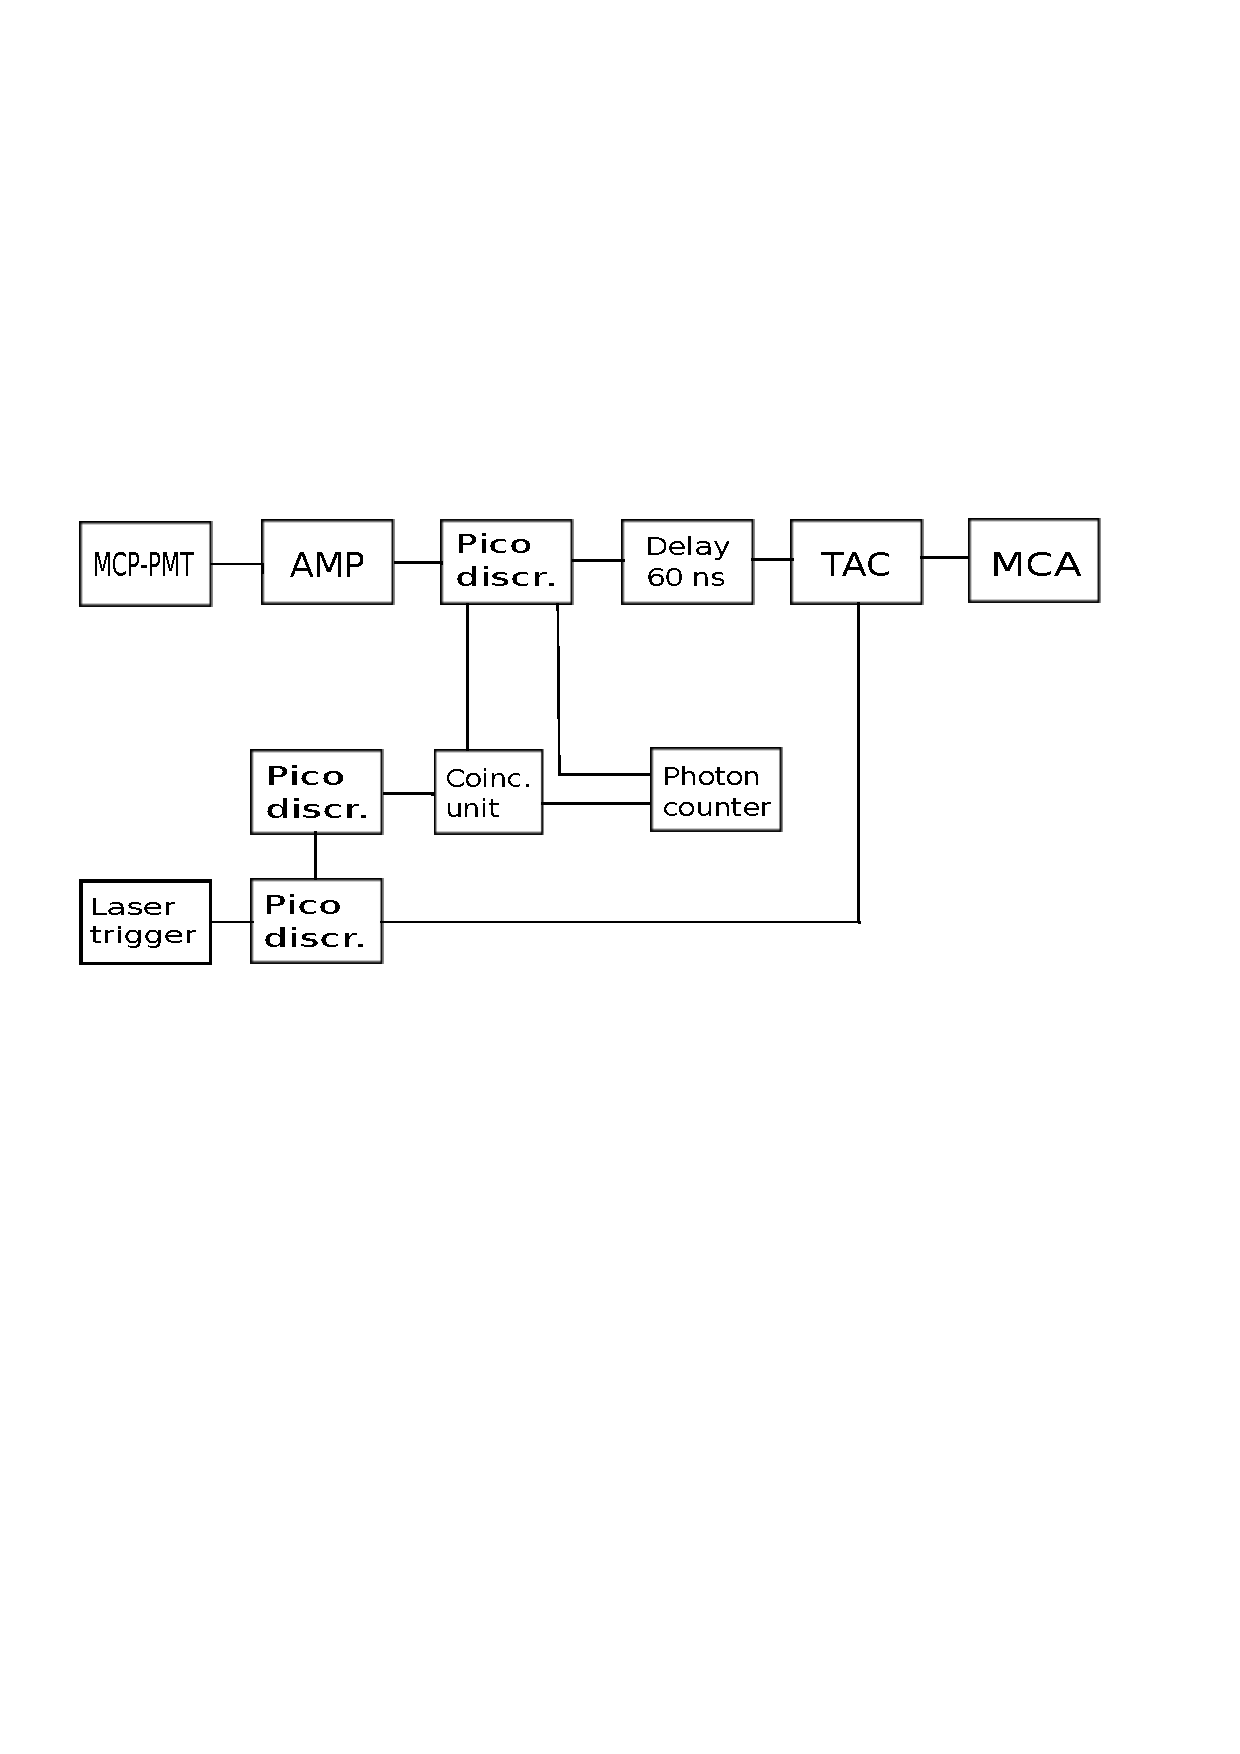
\includegraphics[width=9cm]{../Pictures/Chapter_8/electronics.pdf}
\end{center}
\caption[TCSPC technique]{Principles of time correlated single photon counting (TCSPC)}
\label{fig:daw}
\end{figure}
Thus the main components of a TCPSC system are
\begin{itemize}
\item an excitation system for the sample with an extracted trigger
\item a fluorescent sample with a characteristics periodic light emission
\item a detection system able to extract the time stamps of the arriving single photons.
\end{itemize}
The main sources of error and incertitude on the measured curve are presented in this chapter and can be roughly cathegorized as:
\begin{itemize}
\item the time structure of the excitation
\item the single photon time resolution of the detection system
\item the rate of arrival of optical photons at the stop detector
\item the accumulation times: statistics
\end{itemize}

\subsection{Excitation}
% 


\subsection{Detection}

\section{Data analysis techniques}


\subsection{Iterative reconvolution}
In time correlated single photon counting experiments the problem at hand is statistically speaking to estimate or more parameters (the lifetimes) from a dataset.

The maximum likelihood method is considered to be the most powerful method of parameter estimation.
Consider $n$ independents observation (counts in this case) c$_{1}$, ... , c$_{n}$ and a vector of parameters \textbf{$\theta$} = $(\theta _{1},...\theta _{m})$. If the probability of having the observation i is $p(c_{i}|\theta)$, the likelihood function is
\begin{equation}
L(c_{1},...c_{n}|\theta) = \prod _{i = 1} ^{n} p(c_{i}|\theta) 
\end{equation}
The Maximum Likelihood method provides then an estimate of the true parameters' value as the vector \textbf{$\theta$} that maximizes the likelihood function.
In the case of time correlated single photon counting it is natural to assume that the observed counts $c_{i}$ follow a Poisson distribution
\begin{equation}
p(c_{i}|\theta) = \exp{ \left( -<c_{i}>\right) }\frac{<c_{i}>^{c_{i}}}{c_{i}!}
\end{equation}
where $<c_{i}>$ is the expected value of the number of counts in the i-channel.
This expected value is given by the model taken in to consideration: in this case we can make use of the equations optained in chapter 3. The pdf for the time stamps is given by
\begin{equation}
p_{t_{n}}(t|\theta) = A \cdot \sum _{i} \frac{S_{i}}{\tau _{d,i} - \tau _{r,i}} \cdot \left[ a_{\tau _{d, i}}(t|\theta) - a_{\tau _{r,i}}(t|\theta)\right]
\end{equation}
where 
\begin{eqnarray}
a _{\tau}(t|\theta) &=& \frac{1}{2} \exp{\left(\frac{\sigma _{SPTR} ^{2} - 2t\tau +2\theta \tau + 2t_{TT}\tau}{2\tau ^{2}}\right)} \\
&& \cdot \left[ erf\left( \frac{t-\theta -t_{TT} - \frac{\sigma ^{2}_{SPTR}}{\tau}}{\sigma _{SPTR}\sqrt{2}} \right) + erf \left( \frac{t_{TT}+\frac{\sigma ^{2} _{SPTR}}{\tau}}{\sigma _{SPTR}\sqrt{2}} \right) \right]
\end{eqnarray}
Thus the expected number of counts for the i-channel is
\begin{equation}
<c_{i}> = \int _{(i-1)\Delta} ^{i\Delta} p_{t_{n}}(t|\theta)dt + b_{i} = g _{i}(\theta)
\end{equation}
where $\Delta$ is the time channel width and $b_{i}$ accounts for the average number of dark counts in the channel i.
The vector of parameters \textbf{$\theta$} is given by the lifetimes $\tau _{i}$, the relative intensities $S_{i}$ and a zero time shift $\delta$.
It is customary to determine the best estimate for \textbf{$\theta$} by minimizing the function $-ln(L)$ since the log-likelihood function attains its maximum for the same value as the likelihood function.
In the specific case the function to minimize is
\begin{equation}
-Ln(L) = - \prod _{i=1}^{n} \exp{-g_{i}} \frac{g_{i}^{c_i}}{c_{i}!} = \sum _{i=1}^{n} -g_{i} + c_{i}ln(g_{i}) - ln(c_{i}!)
\end{equation}
which is equivalent to minimizing the Poisson deviance\cite{Bajzer1991}
\begin{equation}
f = \sum _{i=1}^{n} -g_{i} + c_{i}ln(g_{i})
\end{equation}
The standard function minimized in standard fluorescence analysis is usually the $\chi ^{2}$ defined as
\begin{equation}
\chi ^{2} = \sum _{i=1}^{n} \frac{\left[ c_{i} - g_{i}(\theta) \right] ^{2}}{c_{i}}
\end{equation}
or, in the modified least square method\cite{Bajzer1991}
\begin{equation}
\chi _{m}^{2} = \sum _{i=1}^{n} \frac{\left[ c_{i} - g_{i}(\theta) \right] ^{2}}{g_{i}}
\end{equation}
When the number of counts is large they are numerically very close, since the Poisson distribution can be approximated by the Gaussian. Nevertheless in the data analysis the maximum likelihood estimator will be used, since it is preferable the more the low-count region of the decay influences the estimated parameters\cite{Bajzer1991}. 

\subsection{Sources of error}

%% qui il bias
%
%\begin{equation}
%P(m;\epsilon) = \epsilon ^{m} e ^{-\epsilon} / m!
%\end{equation}
%
%\begin{equation}
%Event_{unbias} = U = P(1;\epsilon) = \epsilon e ^{-\epsilon}
%\end{equation}
%
%\begin{equation}
%Event_{bias} = B = \sum _{m = 2} ^{\infty} P(m;\epsilon) \sim \epsilon ^{2} e ^{-\epsilon} / 2
%\end{equation}
%
%$B/U \sim \epsilon / 2$
%
%\begin{equation}
%P(m;\epsilon)P(any < DT) = \frac{\epsilon ^{m} e^{-\epsilon}}{m!}(1-exp(-(\frac{m!\delta}{2(m-2)!})))
%\end{equation}
%
%\begin{equation}
%P(m;\epsilon)P(none < DT) = \frac{\epsilon ^{m} e^{-\epsilon}}{m!}exp(-(\frac{m!\delta}{2(m-2)!}))
%\end{equation}
%
%\begin{equation}
%B/U = \frac{\sum _{2} ^{\infty} mP(m;\epsilon)P(any < DT)}{\sum _{1} ^{\infty} mP(m;\epsilon)P(none < DT)}
%\end{equation}


%\begin{equation}
%F_{hj} = \sum _{i}\frac{1}{y_{i}}\frac{\delta y_{i}}{\delta \alpha _{h}}\frac{\delta y_{i}}{\delta \alpha _{j}}
%\end{equation}
%
%\begin{equation}
%P(n, \alpha _{1}, \alpha _{2},...) = \frac{N!}{n_{1}!...n_{k}!} p_{1}^{n_{1}}\cdot ... \cdot p_{k}^{n_{k}}
%\end{equation}
%
%\begin{equation}
%(F^{multi})_{hj} = \sum _{i} \frac{1}{Np_{i}}\frac{\delta Np_{i}}{\delta \alpha _{h}}\frac{\delta Np_{i}}{\delta \alpha _{j}} = N\sum _{i}\frac{1}{p_{i}}\frac{\delta p_{i}}{\delta \alpha _{h}}\frac{\delta p_{i}}{\delta \alpha _{j}}
%\end{equation}
%
%\begin{equation}
%var_{N}(\tau) = (F^{m})^{-1}=\frac{1}{N}[F^{m}(N=1)]^{-1}
%\end{equation}
%
%\begin{equation}
%N > \frac{var_{1}(\tau)}{required variance (\tau)}
%\end{equation}
%
%%appendice sulla Poisson
%
%\begin{equation}
%p_{i} = \int _{\Delta T_{i}} f(t)dt
%\end{equation}
%
%\begin{equation}
%f(t, \tau , T) = \frac{1}{\tau} exp(-t/tau)\frac{1}{1-exp(-T/tau)} 
%\end{equation}
%
%\begin{equation}
%p_{i}(t, \tau, T) = \int _{(i-1)T/k} ^{iT/k} f(t, \tau, T)dt = frac{exp(\frac{T}{\tau k}) - 1}{1-exp(- t/\tau)} \cdot exp(-\frac{iT}{\tau k})
%\end{equation}
%
%\begin{equation}
%f(t, \tau _{R}, \tau _{D}, T) = [exp(-t/tau _{D}) - exp (-t/tau _{R})] \frac{1}{\tau _{R}[exp(-T\tau _{R})-1] - \tau _{D}[exp(-T\tau _{D})-1]}  
%\end{equation}
%
%


\section{Simulations}